\documentclass[tikz, preview]{standalone}

\usepackage{tikz}
\usepackage[all,2cell]{xy}
\usetikzlibrary{matrix,arrows,shapes,decorations.markings,decorations.pathreplacing}
\definecolor{rewritecolor}{rgb}{0,.9,1}
\tikzset{rewritenode/.style={shape=circle,fill=rewritecolor,scale=0.25,font=\Huge}}
\tikzset{RWopen/.style={shape=circle,draw=black,fill=white,scale=0.5,font=\Huge}}
\tikzset{RWclosed/.style={shape=circle,fill=black,scale=0.5,font=\Huge}}
\tikzset{CDnode/.style={shape=circle,fill=white,scale=.5}}
\tikzset{zxgreen/.style={shape=circle,draw,thick,fill=green}}
\tikzset{zxred/.style={shape=circle,draw,thick,fill=red}}
\tikzset{zxyellow/.style={shape=rectangle,draw,thick,fill=yellow}}
\tikzset{zxdiamond/.style={shape=diamond,star points=5,thick,fill=black,scale=1}}
\tikzset{->-/.style={decoration={markings,mark=at position .5 with {\arrow{>}}},postaction={decorate}}}

\begin{document}

\[
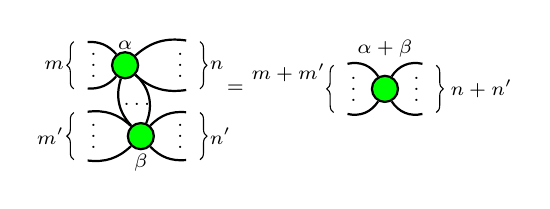
\begin{tikzpicture}
%
%
%
\begin{scope}[shift={(-0.2,0)}] 
\node [zxgreen,label={[shift={(0,-0.1)}]\scriptsize $\alpha$}] (000) at (-0.3,1.2) {};
\node [zxgreen,label={[shift={(0,-0.75)}] \scriptsize $\beta$}] (001) at (-0.1,0.3) {};
\node (v1) at (-0.9,1.5) {};
\node (v2) at (-0.9,0.9) {};
\node (v3) at (-0.9,0.6) {};
\node (v4) at (-0.9,0) {};
\draw  (000) edge[thick,bend right=25] (v1);
\draw  (000) edge[thick,bend left=25] (v2);
\draw  (001) edge[thick,bend right=25] (v3);
\draw  (001) edge[thick,bend left=25] (v4);
%
\node (v5) at (0.6,1.5) {};
\node (v6) at (0.6,0.9) {};
\node (v7) at (0.6,0.6) {};
\node (v8) at (0.6,0) {};
\draw  (000) edge[thick,bend left=25] (v5);
\draw  (000) edge[thick,bend right=25] (v6);
\draw  (001) edge[thick,bend left=25] (v7);
\draw  (001) edge[thick,bend right=25] (v8); 
%
\node (d3) at (0.4,1.3) {\scriptsize $\vdots$};
\node (d4) at (0.4,0.4) {\scriptsize $\vdots$};
\node (d5) at (-0.7,1.3) {\scriptsize $\vdots$};
\node (d5) at (-0.7,0.4) {\scriptsize $\vdots$};
\node at (-0.15,0.7) {\scriptsize $\dots$};
\draw  (000) edge[thick,bend right=30] (001);
\draw  (000) edge[thick,bend left=35] (001);
\draw[decoration={brace,mirror,raise=5pt},decorate]
(v1.east) -- node[left=5pt] {\scriptsize $m$} (v2.east); 
\draw[decoration={brace,mirror,raise=5pt},decorate]
(v3.east) -- node[left=5pt] {\scriptsize $m'$} (v4.east); 
\draw[decoration={brace,raise=5pt},decorate]
(v5.west) -- node[right=5pt] {\scriptsize $n$} (v6.west); 
\draw[decoration={brace,raise=5pt},decorate]
(v7.west) -- node[right=5pt] {\scriptsize $n'$} (v8.west); 
\end{scope}
%
%
%
\node (equal) at (0.9,0.9) {\scriptsize $=$};
%
%
%
\begin{scope}[shift={(0.4,0)}]
\node [zxgreen,label={[shift={(0,0.1)}]\scriptsize $\alpha+\beta$}] (000) at (2.4,0.9) {};
\node (v9) at (1.8,1.2) {};
\node (v10) at (1.8,0.6) {};
\node (v11) at (3,1.2) {};
\node (v12) at (3,0.6) {};
\node (d1) at (2,1) {\scriptsize $\vdots$};
\node (d2) at (2.8,1) {\scriptsize $\vdots$};
%
\draw  (000) edge[thick,bend right=35] (v9);
\draw  (000) edge[thick,bend left=35] (v10);
\draw  (000) edge[thick,bend left=35] (v11);
\draw  (000) edge[thick,bend right=35] (v12);
\draw[decoration={brace,mirror,raise=5pt},decorate]
(v9.east) -- node[shift={(-.75,0.2)}] {\scriptsize $m+m'$} (v10.east); 
\draw[decoration={brace,raise=5pt},decorate]
(v11.west) -- node[shift={(.75,0)}] {\scriptsize $n+n'$} (v12.west); 
\end{scope}
\end{tikzpicture}
\]



\end{document}
